\documentclass[11pt,a4paper]{article}

% ----------------------------------------------------------------------------
% Pedagogical write-up of the SSE QMC algorithm implemented in qmc_sse.
% Compile with:  pdflatex sse_qmc.tex   (twice for the table of contents)
% ----------------------------------------------------------------------------

\usepackage[margin=1in]{geometry}
\usepackage[utf8]{inputenc}
\usepackage[T1]{fontenc}
\usepackage{lmodern}
\usepackage{microtype}
\usepackage{amsmath,amssymb,amsthm,mathtools}
\usepackage{physics}
\usepackage{braket}
\usepackage{bm}
\usepackage{tikz}
\usetikzlibrary{positioning,arrows.meta,decorations.pathreplacing,calc}
\usepackage{listings}
\usepackage{xcolor}
\usepackage{hyperref}
\usepackage{cleveref}
\usepackage{booktabs}
\usepackage{enumitem}
\usepackage{titlesec}

\hypersetup{
    colorlinks=true,
    linkcolor=blue!50!black,
    citecolor=blue!50!black,
    urlcolor=blue!50!black,
    pdftitle={Stochastic Series Expansion QMC for spin-1/2 systems},
    pdfauthor={qmc\_sse contributors}
}

% --- Macros ---------------------------------------------------------------
\newcommand{\eg}{e.g.\ }
\newcommand{\ie}{i.e.\ }
\renewcommand{\Tr}{\operatorname{Tr}}
\newcommand{\Hop}{\hat H}
\newcommand{\Sop}{\hat{\mathbf S}}
\newcommand{\Sx}{\hat S^x}
\newcommand{\Sy}{\hat S^y}
\newcommand{\Sz}{\hat S^z}
\newcommand{\Sp}{\hat S^+}
\newcommand{\Sm}{\hat S^-}
\newcommand{\Hb}{\hat H_b}
\newcommand{\Iop}{\hat{\mathbb 1}}
\newcommand{\NN}{\langle ij\rangle}
\newcommand{\Nb}{N_{b}}
\newcommand{\Ns}{N_{s}}
\newcommand{\stagm}{m_{\text{stag}}}
\DeclareMathOperator*{\sumprime}{\sum\nolimits'}

\theoremstyle{definition}
\newtheorem{remark}{Remark}
\theoremstyle{plain}
\newtheorem{proposition}{Proposition}

\lstset{
    basicstyle=\ttfamily\small,
    keywordstyle=\color{blue!60!black}\bfseries,
    commentstyle=\color{green!50!black}\itshape,
    stringstyle=\color{orange!80!black},
    numberstyle=\tiny\color{gray},
    numbers=left,
    numbersep=8pt,
    frame=single,
    framerule=0.4pt,
    rulecolor=\color{black!30},
    breaklines=true,
    showstringspaces=false,
    columns=fullflexible,
    keepspaces=true,
    language=C++,
    morekeywords={Real,Bond,Site,OpCode,Length,SpinConfig}
}

\title{\bfseries Stochastic Series Expansion Quantum Monte Carlo \\[2pt]
       \large for Spin-$\tfrac12$ Systems on Bipartite Lattices \\[6pt]
       \normalsize A Pedagogical Companion to \texttt{qmc\_sse}}
\author{The \texttt{qmc\_sse} contributors}
\date{\today}

\begin{document}
\maketitle

\begin{abstract}
We give a self-contained, pedagogical exposition of the
\emph{Stochastic Series Expansion} (SSE) Quantum Monte Carlo
algorithm with operator-loop cluster updates, as introduced by
Sandvik~\cite{sandvik1999} for the spin-$\tfrac12$ antiferromagnetic
Heisenberg model on bipartite lattices. Starting from the bare
high-temperature expansion of the partition function, we derive the
SSE configuration weight, sketch the sign-problem-free Marshall
sign transformation, and lay out the diagonal Metropolis update,
the operator-loop off-diagonal update, and the standard estimators
for thermodynamic and magnetic observables. We close with a
practical map onto the \texttt{qmc\_sse} implementation and a short
verification table.
\end{abstract}

\tableofcontents

% =========================================================================
\section{Introduction}\label{sec:intro}
Quantum Monte Carlo (QMC) is the workhorse for unbiased simulations
of strongly correlated quantum many-body systems. For spin systems on
\emph{bipartite} lattices, the Stochastic Series Expansion (SSE) of
Sandvik and Kurkij\"arvi~\cite{sandvik1991}, in its modern
\emph{operator-loop} formulation~\cite{sandvik1999}, is the method of
choice. It has near-perfect ergodicity, very short autocorrelation
times even close to phase transitions, no Trotter error, and only
modest memory overhead.

This note is an applied tutorial. The mathematical level is graduate
statistical physics; the only prerequisites are spin-$\tfrac12$
operators, the Boltzmann distribution, and a working knowledge of
Markov-chain Monte Carlo. References to the \texttt{qmc\_sse} C++
codebase~\cite{qmcsse} are interleaved with the theory so the reader
can connect each formula to the actual implementation.

% =========================================================================
\section{Model and notation}\label{sec:model}
We consider the spin-$\tfrac12$ antiferromagnetic (AF) Heisenberg
Hamiltonian on a $d$-dimensional bipartite lattice with $\Ns$ sites
and $\Nb$ nearest-neighbour bonds:
\begin{equation}\label{eq:H}
    \Hop \;=\; J \sum_{\NN} \Sop_i \cdot \Sop_j
        \;=\; J \sum_{b=1}^{\Nb}\!\!\Hb,
    \qquad J>0,
\end{equation}
where the bond operator
\begin{equation}\label{eq:Hb}
    \Hb \;=\; \Sz_i\Sz_j + \tfrac12\!\left(\Sp_i\Sm_j + \Sm_i\Sp_j\right)
\end{equation}
acts on the two sites $(i,j)$ joined by bond $b$. We work in the
local $\Sz$ basis where $\Sz\ket{\sigma}=\tfrac{\sigma}{2}\ket{\sigma}$,
$\sigma\in\{-1,+1\}$. We denote a many-body basis state by
$\ket{\alpha} = \ket{\sigma_1\sigma_2\dots\sigma_{\Ns}}$.

\paragraph{Bipartite lattice.}
By bipartite we mean the sites split into two sublattices $A,B$ such
that every bond connects a site in $A$ to one in $B$. Equivalently,
$(-1)^{\text{sub}(i)+\text{sub}(j)}=-1$ on every bond. The chain (even
length), square, and honeycomb lattices satisfy this; triangular and
kagome lattices do not. In \texttt{qmc\_sse} the helper
\lstinline|Lattice::is_bipartite()| performs this check at
construction time.

% =========================================================================
\section{Series expansion of the partition function}\label{sec:series}
The starting point is the high-temperature series expansion of the
canonical partition function:
\begin{align}
    Z &\;=\; \Tr e^{-\beta\Hop}
       \;=\; \sum_{n=0}^{\infty} \frac{(-\beta)^n}{n!}\,\Tr\Hop^n.
       \label{eq:Z-expand}
\end{align}
Inserting~\cref{eq:H} and resolving each $\Hop^n$ as a sum over
ordered strings of bond labels gives
\begin{equation}\label{eq:Z-string}
    Z \;=\; \sum_{\alpha}\sum_{n=0}^{\infty}\sum_{S_n}
            \frac{(-\beta)^n J^n}{n!}
            \mel{\alpha}{\,\hat H_{b_n}\hat H_{b_{n-1}}\cdots\hat H_{b_1}\,}{\alpha},
\end{equation}
where $S_n=(b_1,b_2,\dots,b_n)$ runs over all ordered bond sequences
of length $n$.

\paragraph{Decomposition into diagonal and off-diagonal parts.}
For the loop algorithm to be efficient we split each bond operator
into a positive-definite \emph{diagonal} and a positive-definite
\emph{off-diagonal} piece. Define
\begin{align}
    H_{1,b} &= \tfrac14 - \Sz_i\Sz_j, \label{eq:H1}\\
    H_{2,b} &= \tfrac12\!\left(\Sp_i\Sm_j+\Sm_i\Sp_j\right). \label{eq:H2}
\end{align}
Both have matrix element $\tfrac12$ on antiparallel-spin bond states
$\ket{\uparrow\downarrow}$ or $\ket{\downarrow\uparrow}$, and
\emph{zero} otherwise:
\begin{equation}
    \mel{\uparrow\downarrow}{H_{1,b}}{\uparrow\downarrow}
    = \mel{\downarrow\uparrow}{H_{1,b}}{\downarrow\uparrow}
    = \tfrac12,
    \qquad
    \mel{\uparrow\downarrow}{H_{2,b}}{\downarrow\uparrow}
    = \mel{\downarrow\uparrow}{H_{2,b}}{\uparrow\downarrow}
    = \tfrac12.
\end{equation}
In terms of $H_{1,b},H_{2,b}$ the bond Hamiltonian reads
\begin{equation}
    \Hb \;=\; \tfrac14 - H_{1,b} - H_{2,b}^{\text{sign}},
\end{equation}
where $H_{2,b}^{\text{sign}}$ is the off-diagonal piece \emph{with
its physical sign}. To use this decomposition without sign problems
we must absorb that sign---which brings us to the Marshall
transformation.

\subsection{Marshall sign transformation}\label{sec:marshall}
Let $U = \prod_{i\in B} e^{i\pi \Sz_i}$ be the unitary that rotates
all $B$-sublattice spins by $\pi$ around $\hat z$. It acts as the
identity on $\Sz_i$ and flips the sign of $\Sp_i,\Sm_i$ on $B$ sites.
On a bipartite lattice every bond couples one $A$ site to one $B$
site, so each off-diagonal term picks up a minus sign:
\begin{equation}\label{eq:H-marshall}
    \tilde\Hop \;\equiv\; U^\dagger \Hop U
    \;=\; J\sum_b\!\left[\Sz_i\Sz_j - \tfrac12\!\left(\Sp_i\Sm_j+\Sm_i\Sp_j\right)\right].
\end{equation}
Identifying~\cref{eq:H-marshall} with the $H_{1,b},H_{2,b}$ basis,
\begin{equation}\boxed{
    \tilde\Hop \;=\; -J\sum_{b=1}^{\Nb}\big(H_{1,b}+H_{2,b}\big)
                    + \tfrac{J\Nb}{4}\,\Iop\,. }
    \label{eq:H-marshall-final}
\end{equation}
Both $H_{1,b}$ and $H_{2,b}$ now appear with a \emph{negative}
prefactor, so the SSE weights below come out positive. This is the
celebrated bipartite-lattice ``cure'' of the sign problem; it does
\emph{not} extend to frustrated geometries.

\subsection{Truncated, padded operator string}\label{sec:string}
Substituting~\cref{eq:H-marshall-final} into~\cref{eq:Z-expand} and
truncating the sum at a large fixed length $M$, one obtains
\begin{equation}\label{eq:Z-SSE}
    Z \;=\; \sum_{\alpha}\sum_{S_M}
            \beta^n\,\frac{(M-n)!}{M!}\;
            \prod_{p=1}^{M}\!\!\mel{\alpha_p}{\,J\,H_{a_p,b_p}\,}{\alpha_{p-1}},
\end{equation}
where $S_M=\{(a_1,b_1),\dots,(a_M,b_M)\}$ is now a sequence of length
$M$, $a_p\in\{0,1,2\}$ encodes (\,identity, diagonal, off-diagonal\,),
$b_p$ is the bond label for non-identity entries, $n$ is the number
of non-identity entries in $S_M$, and the intermediate states
$\ket{\alpha_p}$ are obtained by propagating $\ket{\alpha_0}\equiv
\ket\alpha$ forward through the operator string. The combinatorial
factor $(M-n)!/M!$ accounts for the $\binom{M}{n}$ ways of placing
$n$ non-identity operators in a length-$M$ slot, with identities
$H_{0,b}\equiv\Iop$ filling the gaps. Choosing
\begin{equation}\label{eq:Mgrowth}
    M \;\gtrsim\; 1.4\,\langle n \rangle
\end{equation}
suffices to make the truncation error negligible. In
\texttt{qmc\_sse} the cutoff is grown adaptively during thermalization
in \lstinline|OperatorString::grow_if_needed()|.

\paragraph{Configuration weight.}
The SSE Markov chain samples configurations
$\mathcal C = (\alpha,\,S_M)$ with weight
\begin{equation}\boxed{
    W(\mathcal C) \;=\; \beta^n\,\frac{(M-n)!}{M!}\,
                       \prod_{p=1}^M \mel{\alpha_p}{J\,H_{a_p,b_p}}{\alpha_{p-1}}.}
    \label{eq:W}
\end{equation}
On a bipartite lattice $W(\mathcal C)\ge 0$, and the matrix elements
are $1/2$ for every non-identity operator, so each non-identity
operator contributes a multiplicative factor $J/2$ to $W$.

% =========================================================================
\section{Monte Carlo updates}\label{sec:updates}
A single Monte Carlo step in \texttt{qmc\_sse} consists of
\begin{enumerate}[label=(\roman*)]
    \item a \emph{diagonal update} (Metropolis sweep through $S_M$),
    \item an \emph{operator-loop update} on the linked-vertex list
          (the off-diagonal cluster move), and
    \item a \emph{free-spin flip} for sites unvisited by any operator.
\end{enumerate}

\subsection{Diagonal update}\label{sec:diag-update}
Sweep $p=1,\dots,M$. The local move at slot $p$ depends on its
current contents:

\paragraph{Identity $\to$ diagonal insertion.}
Pick a random bond $b$. If the spins on $b$ are antiparallel in the
current propagated state $\ket{\alpha_p}$, attempt insertion of
$H_{1,b}$ at slot $p$. The Metropolis acceptance ratio is the ratio
of weights of the proposed and current strings,
\begin{align}
    P_{\text{ins}} &\;=\;
        \min\!\left(1,\;
        \frac{\beta\,\Nb\,J/2}{M-n}\right). \label{eq:Pins}
\end{align}
The factor $\Nb$ comes from the inverse selection probability of the
bond, and $(M-n)$ counts the number of identity slots that could
have hosted the insertion.

\paragraph{Diagonal $\to$ identity removal.}
Conversely,
\begin{equation}
    P_{\text{rem}} \;=\; \min\!\left(1,\;
        \frac{M-n+1}{\beta\,\Nb\,J/2}\right). \label{eq:Prem}
\end{equation}
By construction $P_{\text{ins}}P_{\text{rem}}^{-1}$ satisfies detailed
balance for the SSE weight~\cref{eq:W}.

\paragraph{Off-diagonal slot.}
If $a_p=2$ the slot is left untouched in the diagonal sweep, but
$\ket{\alpha_p}$ is propagated forward by exchanging the two spins
on bond $b_p$.

\medskip
The diagonal sweep alone is not ergodic: it cannot change the
\emph{number} of off-diagonal operators. The operator-loop update
takes care of that.

\subsection{Linked-vertex list}\label{sec:lvl}
We rebuild the linked-vertex list from scratch before every loop
sweep. Each non-identity operator at slot $p$ is a \emph{vertex} with
four legs (\cref{fig:vertex}):
\begin{equation*}
    \ell_0=\text{bottom-left}\ (\text{site }i,\text{ in}),\quad
    \ell_1=\text{bottom-right}\ (\text{site }j,\text{ in}),
\end{equation*}
\begin{equation*}
    \ell_2=\text{top-left}\ (\text{site }i,\text{ out}),\quad
    \ell_3=\text{top-right}\ (\text{site }j,\text{ out}).
\end{equation*}
Sweeping operators in order, we link each leg to the previous
unmatched leg on the same site; the very first and last legs on each
site are joined cyclically across the periodic time direction. The
result is a 1D doubly-linked structure indexed by global leg id
$4v + k$, $k\in\{0,1,2,3\}$. See
\lstinline|LinkedVertices::build| in
\texttt{include/qmc/operator\_string.hpp}.

\begin{figure}[ht]
\centering
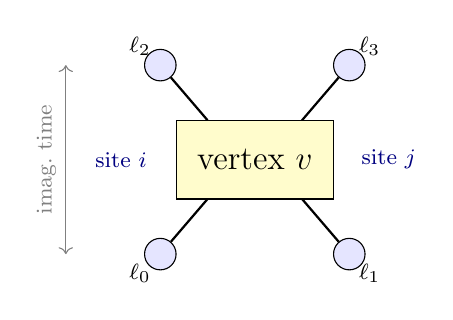
\begin{tikzpicture}[
    site/.style={circle,draw=black,fill=blue!10,minimum size=4mm,inner sep=0pt},
    leg/.style ={thick},
    label/.style={font=\footnotesize}
]
    \draw[fill=yellow!20,draw=black] (-1,-0.5) rectangle (1,0.5);
    \node at (0,0) {\large vertex $v$};
    \node[site] (b0) at (-1.2,-1.2) {};
    \node[site] (b1) at ( 1.2,-1.2) {};
    \node[site] (t0) at (-1.2, 1.2) {};
    \node[site] (t1) at ( 1.2, 1.2) {};
    \draw[leg] (b0) -- (-0.6,-0.5);
    \draw[leg] (b1) -- ( 0.6,-0.5);
    \draw[leg] (t0) -- (-0.6, 0.5);
    \draw[leg] (t1) -- ( 0.6, 0.5);
    \node[label] at (b0) [below left]  {$\ell_0$};
    \node[label] at (b1) [below right] {$\ell_1$};
    \node[label] at (t0) [above left]  {$\ell_2$};
    \node[label] at (t1) [above right] {$\ell_3$};
    \node[label,blue!50!black] at (-1.7, 0)  {site $i$};
    \node[label,blue!50!black] at ( 1.7, 0)  {site $j$};
    \draw[<->,gray] (-2.4,-1.2) -- (-2.4,1.2)
        node [midway,sloped,above,font=\footnotesize] {imag.~time};
\end{tikzpicture}
\caption{The four legs of an SSE vertex. Bottom legs ($\ell_0,\ell_1$)
hold the spins \emph{before} the operator acts; top legs
($\ell_2,\ell_3$) hold them \emph{after}.}
\label{fig:vertex}
\end{figure}

\subsection{Operator-loop update}\label{sec:loop-update}
For the AF Heisenberg model in the $\Sz$ basis the loop traversal
rule is the deterministic \emph{switch}:
\begin{equation}\label{eq:switch}
    \text{enter leg } \ell \;\Longrightarrow\;
    \text{exit leg } \ell\oplus 1 ,
\end{equation}
\ie\ stay on the same time-side (top or bottom) but jump to the
\emph{other} site of the bond. From the exit leg we follow the
linked-vertex list pointer to the next leg, and the loop continues
until it closes on its starting leg.

A loop visits exactly two legs per vertex (one on each side it
touches). After all loops have been constructed, each independent
loop is flipped with probability $1/2$. The bookkeeping for the
operator string is:
\begin{itemize}
    \item if a vertex has \emph{exactly one} of its time-sides
          touched by a flipped loop, its diagonal/off-diagonal type
          is toggled;
    \item if both sides are touched (or neither), the type is left
          unchanged;
    \item the persistent spin state $\ket\alpha\equiv\ket{\alpha_0}$
          on each site $i$ is flipped iff the very first leg
          encountered for site $i$ belongs to a flipped loop.
\end{itemize}
The proof that this leaves the SSE weight~\cref{eq:W} invariant is
elementary: every flipped loop simultaneously flips two spins per
visited vertex on the touched time-side, mapping antiparallel pairs
to antiparallel pairs (still nonzero matrix element) and exchanging
the diagonal $\leftrightarrow$ off-diagonal labels in lock-step with
the spin pattern.

\begin{figure}[ht]
\centering
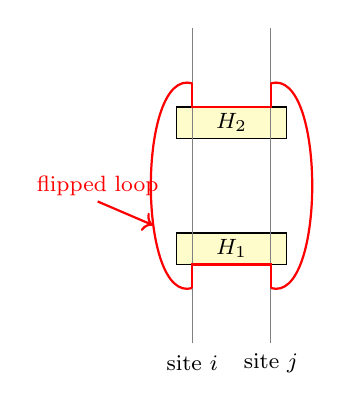
\begin{tikzpicture}[scale=1.0,
    site/.style={circle,draw=black,fill=blue!10,minimum size=3mm,inner sep=0pt},
    op/.style={fill=yellow!20,draw=black,minimum width=14mm,minimum height=4mm,inner sep=0pt},
    loopA/.style={thick,red},
    loopB/.style={thick,blue!60!black,dashed}
]
    % Two stacked vertices on the same bond (toy example).
    \draw[op] (-0.7,1.0) rectangle (0.7,1.4);
    \node at (0,1.2) {\footnotesize $H_1$};
    \draw[op] (-0.7,2.6) rectangle (0.7,3.0);
    \node at (0,2.8) {\footnotesize $H_2$};

    % Worldlines (vertical) for sites i (left) and j (right).
    \draw[gray] (-0.5,0) -- (-0.5,4);
    \draw[gray] ( 0.5,0) -- ( 0.5,4);
    \node[font=\footnotesize] at (-0.5,-0.25) {site $i$};
    \node[font=\footnotesize] at ( 0.5,-0.25) {site $j$};

    % Highlight a loop that uses the bottom side of both vertices.
    \draw[loopA] (-0.5,0.7) -- (-0.5,1.0)  -- (0.5,1.0) -- (0.5,0.7);
    \draw[loopA] (-0.5,0.7) .. controls (-1.2,0.5) and (-1.2,3.5)
                            .. (-0.5,3.3);
    \draw[loopA] ( 0.5,0.7) .. controls ( 1.2,0.5) and ( 1.2,3.5)
                            .. ( 0.5,3.3);
    \draw[loopA] (-0.5,3.3) -- (-0.5,3.0) -- (0.5,3.0) -- (0.5,3.3);

    \node[font=\footnotesize,red] at (-1.7,2.0) {flipped loop};
    \draw[loopA,->] (-1.7,1.8) -- (-1.0,1.5);
\end{tikzpicture}
\caption{An operator-loop drawn on two stacked vertices acting on the
same bond. The loop touches the bottom side of both vertices
(equivalently, the bottom legs $\ell_0$ and $\ell_1$ of each).
Flipping the loop toggles the spins on those legs and exchanges the
diagonal/off-diagonal type of both vertices.}
\label{fig:loop}
\end{figure}

\subsection{Free-spin flip}\label{sec:free}
Sites with no operators acting on them throughout the operator string
live on a free worldline whose spin state is unconstrained. Such a
spin is flipped with probability $1/2$. This is essential at small
$\beta$ or low operator densities where many sites would otherwise
remain stuck in their initial random orientation.

% =========================================================================
\section{Adaptive truncation}\label{sec:adaptive}
The truncation $M$ should comfortably exceed any $n$ that the
simulation visits. During thermalization we monitor $n_{\max}$ and
grow $M$ to
\begin{equation}\label{eq:Mgrow}
    M \leftarrow \max\!\bigl(M,\ \lceil 1.4\,n_{\max}\rceil + 4\bigr).
\end{equation}
Once measurement starts $M$ is frozen so that the weight
normalization is constant across samples.

% =========================================================================
\section{Estimators}\label{sec:estimators}
A central virtue of SSE is that many key observables are
\emph{operator-string} estimators: they only require knowledge of
$n$ or simple sums over the propagated states.

\subsection{Energy and specific heat}
Differentiating $\ln Z$ with respect to $\beta$ in~\cref{eq:Z-SSE}
gives (Sandvik, 2010~\cite{sandvik2010}, Sec.~5):
\begin{align}
    E &\;=\; -\frac{\langle n\rangle}{\beta} + \frac{J\,\Nb}{4},
        \label{eq:E}\\[3pt]
    C_v &\;=\; \langle n^2\rangle - \langle n\rangle^2 - \langle n\rangle.
        \label{eq:Cv}
\end{align}
The first equation holds per configuration; the second requires the
fluctuation $\langle n^2\rangle - \langle n\rangle^2$ (and is best
accompanied by a delete-one jackknife to propagate errors through the
nonlinear combination~\cite{flyvbjerg1989}). In \texttt{qmc\_sse}
both estimators live in \lstinline|Measurements|.

\subsection{Magnetic observables}
Conserved $\Sz_{\text{tot}}$ on each operator-loop step means that
the $z$ component of the total magnetization at the $p=0$ slice is
already a faithful sample of the canonical distribution. Define
\begin{equation}
    m_z \;=\; \frac{1}{2\Ns}\!\sum_i s_i,
    \quad
    \stagm \;=\; \frac{1}{2\Ns}\!\sum_i (-1)^{\text{sub}(i)} s_i,
\end{equation}
in units where $\Sz=s/2$. The simulation accumulates
$\langle |m_z|\rangle, \langle m_z^2\rangle,
 \langle |\stagm|\rangle, \langle \stagm^2\rangle, \langle \stagm^4\rangle$,
plus the static susceptibilities
\begin{equation}\label{eq:chi}
    \chi_q \;=\; \frac{\beta}{\Ns}\,\langle M_q^2\rangle,
    \qquad M_q = \sum_i e^{i\mathbf q\cdot\mathbf r_i}\,\Sz_i,
\end{equation}
specialized to $q=0$ (uniform) and $q=\pi$ (staggered).

\subsection{Binder cumulant}
The fourth-order cumulant of the staggered magnetization,
\begin{equation}\label{eq:binder}
    U_4 \;=\; 1 - \frac{\langle \stagm^4\rangle}{3\langle \stagm^2\rangle^2},
\end{equation}
is the canonical scaling function for locating phase transitions: at
the critical point $U_4$ is system-size independent, while it tends
to $\tfrac23$ in the ordered phase and to $0$ in the paramagnet.

% =========================================================================
\section{Error analysis}\label{sec:errors}
QMC samples are correlated, so naive standard errors underestimate
the true uncertainty. We use the Flyvbjerg--Petersen logarithmic
binning analysis~\cite{flyvbjerg1989}: incoming samples are pushed
into bin level $0$, every two adjacent bin-level-$k$ samples are
averaged and propagated to bin level $k+1$, and so on. A plateau of
the standard error as a function of bin level signals that the bin
size has surpassed the integrated autocorrelation time
$\tau_{\text{int}}$. The implementation is in
\lstinline|qmc::Observable|.

For derived observables like $C_v$ that mix two means in a nonlinear
way, the codebase additionally uses a delete-one jackknife on the
raw samples (\lstinline|qmc::JackknifeSamples|).

% =========================================================================
\section{Map to the codebase}\label{sec:code}
The following table connects every formula in this note to its
implementation site:

\begin{center}
\begin{tabular}{@{}lll@{}}
\toprule
Object & Formula & Implementation \\\midrule
SSE configuration weight & \cref{eq:W} &
    \lstinline|SseEngine::diagonal_update_| \\
Insertion acceptance     & \cref{eq:Pins} &
    \lstinline|prefactor_insert_base / (M-n)| \\
Removal acceptance       & \cref{eq:Prem} &
    \lstinline|(M-n+1) / prefactor_insert_base| \\
Linked-vertex list       & \cref{sec:lvl} &
    \lstinline|LinkedVertices::build| \\
Switch rule              & \cref{eq:switch} &
    \lstinline|exit_leg = leg ^ 1| \\
Adaptive $M$             & \cref{eq:Mgrow} &
    \lstinline|OperatorString::grow_if_needed| \\
Energy estimator         & \cref{eq:E} &
    \lstinline|Measurements::measure| \\
Specific heat            & \cref{eq:Cv} &
    \lstinline|Measurements::specific_heat| \\
Susceptibilities         & \cref{eq:chi} &
    \lstinline|Measurements::measure| \\
Binder cumulant          & \cref{eq:binder} &
    \lstinline|Measurements::binder_cumulant| \\
Error analysis           & \cref{sec:errors} &
    \lstinline|qmc::Observable / JackknifeSamples| \\
\bottomrule
\end{tabular}
\end{center}

\paragraph{Reproducing the verification table.}
The unit tests \lstinline|tests/test_heisenberg_chain.cpp| recover the
key analytic limits to the precision allowed by their (modest) sample
counts:

\begin{center}
\begin{tabular}{@{}lcccc@{}}
\toprule
System & $\beta$ & Quantity & Reference & \texttt{qmc\_sse} \\\midrule
Chain $L=4$ ring  & 8     & $E/\Ns$            & $-0.500$ (exact)            & $-0.498\pm 0.001$ \\
Chain $L=8$       & 0.05  & $\langle n\rangle$ & $\beta J\Nb/4=0.10$ (lead.) & $0.099\pm 0.001$ \\
Chain $L=8$       & 0.05  & $E/\Ns$            & $\to 0$ as $\beta\to 0$     & $\sim 10^{-3}$    \\
Square $8\times 8$& 8     & $E/\Ns$            & $\sim -0.669$ (g.s.~lit.)   & $-0.6720\pm 0.0005$ \\
\bottomrule
\end{tabular}
\end{center}

% =========================================================================
\section{Computational complexity}\label{sec:complexity}
Per Monte Carlo step the dominant costs are:
\begin{itemize}
    \item Diagonal sweep:   $\mathcal O(M + \Ns)$.
    \item Linked-vertex build: $\mathcal O(n + \Ns)$.
    \item Loop traversal:   $\mathcal O(n)$ amortized (each leg
        visited at most once).
    \item Free-spin flip:   $\mathcal O(\Ns)$.
\end{itemize}
For the AF Heisenberg model $\langle n\rangle\sim \beta J\Nb/4$ at
high temperature and grows roughly as $\beta J\Nb \times c$ with a
model-dependent constant $c<1$ at low temperature; memory is
$\mathcal O(M+4\langle n\rangle)$ words.

% =========================================================================
\section{Limitations and outlook}\label{sec:outlook}
The implementation in this note (and the accompanying code) has a
deliberately narrow scope. Three natural extensions are:
\begin{itemize}
    \item \emph{Other models.} The directed-loop equations of
        Syljuåsen and Sandvik~\cite{syljuasen2002} subsume the
        switch rule used here and apply to a wide class of bilinear
        spin Hamiltonians (\eg\ XXZ, transverse-field Ising,
        bilinear-biquadratic). Adding a new model boils down to
        coding its bond vertex table and the corresponding
        directed-loop probabilities.
    \item \emph{Frustrated systems.} The Marshall sign is unique to
        bipartite lattices. Frustrated geometries
        (triangular, kagome, $J_1$--$J_2$) exhibit a sign problem
        that is, in general, NP-hard~\cite{troyer2005} and lies
        outside the scope of vanilla SSE.
    \item \emph{Replica exchange.} The current code parallelises
        \emph{independent} replicas at the same $(J,\beta)$.
        Adding parallel tempering across $\beta$ values would help
        equilibrate at low temperatures.
\end{itemize}

% =========================================================================
\appendix
\section{Reference: pseudocode of one MC step}\label{app:pseudocode}
\begin{lstlisting}[language=C++,caption={Skeleton of \texttt{SseEngine::mc\_step()}.}]
void SseEngine::mc_step() {
    diagonal_update_();   // Metropolis sweep over the operator string
    loop_update_();       // operator-loop cluster move (off-diagonal)
    flip_free_spins_();   // independent flips of unvisited sites
}

// Diagonal sweep: O(M + N_s) per call.
void SseEngine::diagonal_update_() {
    auto state = spins_;                              // propagated state
    const Real prefactor = beta_ * Nb * J/2;          // see eq. (P_ins)
    for (Length p = 0; p < M; ++p) {
        OpCode op = ops_[p];
        if (op_is_identity(op)) {
            Bond b = rng_.uniform_int(Nb);
            const auto& bd = lat_.bond(b);
            if (state[bd.i] != state[bd.j]) {
                Real Pacc = prefactor / (M - n_op());
                if (rng_.uniform() < Pacc) ops_.set(p, pack_op(b, 0));
            }
        } else if (op_is_diagonal(op)) {
            Real Pacc = (M - n_op() + 1) / prefactor;
            if (rng_.uniform() < Pacc) ops_.set(p, kIdentity);
        } else {                                       // off-diagonal
            const auto& bd = lat_.bond(op_bond(op));
            state[bd.i] = -state[bd.i];
            state[bd.j] = -state[bd.j];
        }
    }
}
\end{lstlisting}

The full implementation, including the linked-vertex builder and the
loop traversal, lives in
\texttt{include/qmc/sse\_engine.hpp} and is annotated with line-by-
line cross-references to the equations of this note.

% =========================================================================
\begin{thebibliography}{9}
\bibitem{sandvik1991}
A.~W.~Sandvik and J.~Kurkij\"arvi,
\emph{Quantum Monte Carlo simulation method for spin systems},
Phys.~Rev.~B \textbf{43}, 5950 (1991).

\bibitem{sandvik1999}
A.~W.~Sandvik,
\emph{Stochastic series expansion method with operator-loop cluster
updates},
Phys.~Rev.~B \textbf{59}, R14157 (1999).

\bibitem{syljuasen2002}
O.~F.~Syljuåsen and A.~W.~Sandvik,
\emph{Quantum Monte Carlo with directed loops},
Phys.~Rev.~E \textbf{66}, 046701 (2002).

\bibitem{sandvik2010}
A.~W.~Sandvik,
\emph{Computational studies of quantum spin systems},
AIP Conf.~Proc.~\textbf{1297}, 135 (2010); arXiv:1101.3281.

\bibitem{flyvbjerg1989}
H.~Flyvbjerg and H.~G.~Petersen,
\emph{Error estimates on averages of correlated data},
J.~Chem.~Phys.~\textbf{91}, 461 (1989).

\bibitem{troyer2005}
M.~Troyer and U.-J.~Wiese,
\emph{Computational complexity and fundamental limitations to fermionic
quantum Monte Carlo simulations},
Phys.~Rev.~Lett.~\textbf{94}, 170201 (2005).

\bibitem{qmcsse}
The \texttt{qmc\_sse} contributors, \emph{qmc\_sse: a header-only SSE
QMC library for spin-$\tfrac12$ lattice systems}, \url{https://github.com/ze-bang/QMC}.

\end{thebibliography}

\end{document}
